\begin{figure}
    \centering
    \setlength{\tabcolsep}{1pt}
    \scriptsize{
    \begin{tabular}{cc cccc}
        \multicolumn{2}{c}{\raisebox{22pt}{\rotatebox[origin=t]{90}{Input}}} &
        \includegraphics[width=0.228\linewidth]{images/reconstruction_comparison/0_original.jpg} &
        \includegraphics[width=0.228\linewidth]{images/reconstruction_comparison/1_original.jpg} &
        \includegraphics[width=0.228\linewidth]{images/reconstruction_comparison/graffiti/original.jpg} &
        \includegraphics[width=0.228\linewidth]{images/reconstruction_comparison/pinapple_man/original.jpg} \\
        
        \multicolumn{2}{c}{\raisebox{22pt}{\rotatebox[origin=t]{90}{DDIM Inv.}}} &
        \includegraphics[width=0.228\linewidth]{images/reconstruction_comparison/0_no_ipa.jpg} &
        \includegraphics[width=0.228\linewidth]{images/reconstruction_comparison/1_no_ipa.jpg} &
        \includegraphics[width=0.228\linewidth]{images/reconstruction_comparison/graffiti/recon.jpg} &
        \includegraphics[width=0.228\linewidth]{images/reconstruction_comparison/pinapple_man/recon.jpg} \\
        
        \raisebox{22pt}{\rotatebox[origin=t]{90}{DDIM Inv.}} &
        \raisebox{22pt}{\rotatebox[origin=t]{90}{+ Tight Inversion}} &
        \includegraphics[width=0.228\linewidth]{images/reconstruction_comparison/0_ipa.jpg} &
        \includegraphics[width=0.228\linewidth]{images/reconstruction_comparison/1_ipa.jpg} &
        \includegraphics[width=0.228\linewidth]{images/reconstruction_comparison/graffiti/ipa_recon.jpg} &
        \includegraphics[width=0.228\linewidth]{images/reconstruction_comparison/pinapple_man/recon_ipa.jpg} \\
        
        \multicolumn{2}{c}{\raisebox{22pt}{\rotatebox[origin=t]{90}{ReNoise}}} &
        \includegraphics[width=0.228\linewidth]{images/reconstruction_comparison/0_renoise_bbox.jpg} &
        \includegraphics[width=0.228\linewidth]{images/reconstruction_comparison/1_renoise.jpg} &
        \includegraphics[width=0.228\linewidth]{images/reconstruction_comparison/graffiti/renoise_recon.jpg} &
        \includegraphics[width=0.228\linewidth]{images/reconstruction_comparison/pinapple_man/recon_renoise.jpg} \\
        
        \raisebox{22pt}{\rotatebox[origin=t]{90}{ReNoise}} &
        \raisebox{22pt}{\rotatebox[origin=t]{90}{+ Tight Inversion}} &
        \includegraphics[width=0.228\linewidth]{images/reconstruction_comparison/0_renoise+ipa_bbox.jpg} &
        \includegraphics[width=0.228\linewidth]{images/reconstruction_comparison/1_renoise+ipa.jpg} &
        \includegraphics[width=0.228\linewidth]{images/reconstruction_comparison/graffiti/renoise+ipa_recon.jpg} &
        \includegraphics[width=0.228\linewidth]{images/reconstruction_comparison/pinapple_man/recon_renoise+ipa.jpg} \\
        
        && \multicolumn{4}{c}{\textbf{SDXL}}       
    \end{tabular}
    }
    \caption{Qualitative reconstruction results with SDXL. Integrating Tight Inversion with various inversion methods enhances reconstruction. Observe the reflection on the window in the second column.}
    \label{fig:recon-qualitative-comp-sdxl}
\end{figure}


\section{Experiments}
\label{sec:experiments}
\graphicspath{../images/}


We evaluate our inversion method based on both reconstruction accuracy and editability. To demonstrate editability, we utilize a variety of existing image editing techniques, each excelling in different types of edits, and apply them to the inverted images.

\begin{table}
{\small
    \centering
    \caption{Quantitative comparison of various existing inversion methods with and without Tight Inversion.}
    \vspace{-8pt}
    \setlength{\tabcolsep}{3.5pt}
    \begin{tabular}{l c c c c}
      \toprule
      Method & $L_2$ $\downarrow$ & PSNR $\uparrow$ & SSIM $\uparrow$ & LPIPS $\downarrow$ \\
      \midrule
      DDIM Inversion & 50.5897 & 25.3404 & 0.7699 & 0.1485 \\
      DDIM Inversion + Ours & 42.8394 & 26.9030 & 0.7981 & 0.1055 \\
      \midrule
      ReNoise & 42.9509 & 27.1584 & 0.7928 & 0.1179 \\
      ReNoise + Ours & 37.8595 & 28.0413 & 0.8134 & 0.0877 \\
      \bottomrule
      \end{tabular}
    \label{tab:reconstruction_comparison_quant}
    }
  \end{table}

\begin{figure}
    \centering
    \setlength{\tabcolsep}{1pt}
    \scriptsize{
    \begin{tabular}{cc cccc}
        \multicolumn{2}{c}{\raisebox{22pt}{\rotatebox[origin=t]{90}{Input}}} &
        \includegraphics[width=0.228\linewidth]{images/reconstruction_comparison/flux-portrait-recon0/original.jpg} &
        \includegraphics[width=0.228\linewidth]{images/reconstruction_comparison/flux-portrait-recon1/original.jpg} &
        \includegraphics[width=0.228\linewidth]{images/reconstruction_comparison/flux-portrait-recon2/original.jpg} &
        \includegraphics[width=0.228\linewidth]{images/reconstruction_comparison/flux-portrait-recon3/original.jpg} \\
        
        \multicolumn{2}{c}{\raisebox{22pt}{\rotatebox[origin=t]{90}{RF Inv.}}} &
        \includegraphics[width=0.228\linewidth]{images/reconstruction_comparison/flux-portrait-recon0/reconstruction.jpg} &
        \includegraphics[width=0.228\linewidth]{images/reconstruction_comparison/flux-portrait-recon1/reconstruction.jpg} &
        \includegraphics[width=0.228\linewidth]{images/reconstruction_comparison/flux-portrait-recon2/reconstruction.jpg} &
        \includegraphics[width=0.228\linewidth]{images/reconstruction_comparison/flux-portrait-recon3/reconstruction.jpg} \\
        
        \raisebox{22pt}{\rotatebox[origin=t]{90}{RF Inv.}} &
        \raisebox{22pt}{\rotatebox[origin=t]{90}{+ Tight Inversion}} &
        \includegraphics[width=0.228\linewidth]{images/reconstruction_comparison/flux-portrait-recon0/reconstruction-pulid.jpg} &
        \includegraphics[width=0.228\linewidth]{images/reconstruction_comparison/flux-portrait-recon1/reconstruction_pulid.jpg} &
        \includegraphics[width=0.228\linewidth]{images/reconstruction_comparison/flux-portrait-recon2/reconstruction-pulid.jpg} &
        \includegraphics[width=0.228\linewidth]{images/reconstruction_comparison/flux-portrait-recon3/reconstruction-pulid.jpg} \\
        
        && \multicolumn{4}{c}{\textbf{Flux}}       
    \end{tabular}
    }
    \caption{Qualitative reconstruction results with Flux. Integrating Tight Inversion with RF-Inversion enhances the identity preservation of the reconstruction.}
    \label{fig:recon-qualitative-comp-flux}
\end{figure}


Unless stated otherwise, our experiments use SDXL~\cite{podell2024sdxl} with DDIM scheduler~\cite{song2022denoisingdiffusionimplicitmodels}. All experiments utilize $50$ denoising steps with a default guidance scale of $7.5$. For image conditioning, we employ IP-Adapter-plus\_sdxl\_vit-h~\cite{ye2023ipadaptertextcompatibleimage}.
In few-step diffusion experiments, we use SDXL-Turbo~\cite{sauer2023adversarialdiffusiondistillation} with an Euler scheduler and perform $4$ denoising steps. We also explore Flux~\cite{flux} using FLUX.1-dev where we condition the model with PulID-Flux~\cite{guo2024pulid} and use RF-Inversion~\cite{rout2024rfinversion} with 28 steps. As PulID was trained only on human faces, we focus on this domain for evaluating our method with Flux.


\subsection{Reconstruction}

We evaluate reconstruction both qualitatively and quantitatively. For quantitative evaluation, we measure $L_2$ distance, PSNR, SSIM and LPIPS~\cite{zhang2018perceptual}.
Figures~\ref{fig:motivation-figure} and \ref{fig:recon-qualitative} present qualitative results of DDIM inversion~\cite{dhariwal2021diffusionmodelsbeatgans} under increasingly descriptive conditions. These examples highlight that conditioning the inversion process on an image significantly improves reconstruction in highly detailed regions. Notably, in the third example of Figure~\ref{fig:recon-qualitative}, our method successfully reconstructs the tattoo on the back of the right boxer. Furthermore, the boxer's leg pose is more accurately preserved, and the tattoo on the leg becomes visible.



\vspace{-6pt}
\paragraph{\textbf{Comparisons}}
We integrate Tight Inversion with several existing inversion methods and demonstrate that it enhances their reconstruction performance. Specifically, we combine our method with DDIM inversion~\cite{dhariwal2021diffusionmodelsbeatgans}, ReNoise~\cite{garibi2024renoise}, and RF-Inversion~\cite{rout2024rfinversion}. Note that DDPM-based inversion methods typically guarantee perfect reconstruction, so we compare with these methods only in terms of editability.
Qualitative results are shown in Figures~\ref{fig:recon-qualitative-comp-sdxl} and \ref{fig:recon-qualitative-comp-flux}. As illustrated, integrating Tight Inversion with existing methods consistently improves reconstruction. For example, in Figure~\ref{fig:recon-qualitative-comp-sdxl}, our method accurately reconstructs the handrail in the leftmost example and the man with the blue shirt in the rightmost example.

We further validate the improvement quantitatively. Following previous works~\cite{Mokady_2023_CVPR, garibi2024renoise}, we utilize the test set of MS-COCO~\cite{lin2015microsoftcococommonobjects} and present the results in Table~\ref{tab:reconstruction_comparison_quant}. As observed from the table, our method improves reconstruction of existing inversion methods across all metrics.


\paragraph{\textbf{Ablation Studies}}
We conduct ablation studies to evaluate the importance of combining image conditioning with an inversion method. Since IP-Adapter is trained to reconstruct images from image conditions, it is reasonable to explore whether accurate reconstruction can be achieved solely by conditioning on the image, without requiring a carefully selected noise initialization.
Figure~\ref{fig:ablation1} explores this possibility. In the first row, a random noise is sampled, and the denoising process is conditioned on the input image. While the semantics and colors are captured, the reconstructed image poorly matches the original one. This demonstrates that precise reconstruction still requires a specific initial noise.
In the second row, DDIM inversion is performed using only a text prompt, while denoising is conditioned on the input image. The results show slight over-saturation and the disappearance of the phone in the man's hand.
In the third row, our Tight Inversion method is applied, conditioning both inversion and denoising on an input image. Our method significantly outperforms the alternatives, faithfully reconstructing both colors and fine details, including the phone.


\begin{figure}
    \setlength{\tabcolsep}{1pt}
  \centering
  \begin{tabular}{cccc}
   \raisebox{30pt}{\rotatebox[origin=t]{90}{Random noise}} &
    \includegraphics[width=0.32\linewidth]{images/ipa_method_ablation/random_noise+ipa/original.jpg} &
    \includegraphics[width=0.32\linewidth]{images/ipa_method_ablation/random_noise+ipa/reconstruction.jpg} &
    \includegraphics[width=0.32\linewidth]{images/ipa_method_ablation/random_noise+ipa/a_person_wearing_a_red_hat.jpg} \\
    \raisebox{30pt}{\rotatebox[origin=t]{90}{DDIM Inversion}} &
    \includegraphics[width=0.32\linewidth]{images/ipa_method_ablation/ipa_denoising_only/original.jpg} &
    \includegraphics[width=0.32\linewidth]{images/ipa_method_ablation/ipa_denoising_only/reconstruction.jpg} &
    \includegraphics[width=0.32\linewidth]{images/ipa_method_ablation/ipa_denoising_only/a_person_wearing_a_red_hat.jpg} \\
    \raisebox{30pt}{\rotatebox[origin=t]{90}{Tight Inversion}} &
    \includegraphics[width=0.32\linewidth]{images/ipa_method_ablation/ipa_inversion+denoising/original.jpg} &
    \includegraphics[width=0.32\linewidth]{images/ipa_method_ablation/ipa_inversion+denoising/reconstruction.jpg} &
    \includegraphics[width=0.32\linewidth]{images/ipa_method_ablation/ipa_inversion+denoising/a_person_wearing_a_red_hat.jpg} \\
    & Input & Reconstruction & $+$ ``a red hat'' \\
  \end{tabular}
  \caption{In all three rows, the denoising process is conditioned on the input image. In the first row, a random noise is sampled instead of inverting the image. In the second row, we apply vanilla DDIM inversion conditioned on a text prompt only. In the third row, we apply Tight Inversion, conditioning both the inversion and the denoising process on the input image. }
  \label{fig:ablation1}
\end{figure}


We further explore the impact of image conditioning strength. Specifically, IP-Adapter provides a guidance scale, $s$, which controls the influence of the input image on the generated output. Setting $s$ to zero is equivalent to using the text-to-image model without IP-Adapter. Figure~\ref{fig:ablation2} presents the results for different values of $s$.
As expected, we observe that reconstruction quality (second row) improves with higher IP-Adapter scales, emphasizing the importance of precise conditioning.



\begin{table}[H]
\caption{Comparison of ClipScore with the selected LoRA integration methods under different number of LoRAs.}
\label{ablation2}
\begin{center}
\scalebox{0.8}{
\begin{tabular}{c|cccc}
\toprule
Model & ClipScore (N=2) & ClipScore (N=3) & ClipScore (N=4) & ClipScore (N=5) \\
\midrule
CMLoRA ($\text{Cache}_{D}$) & \textcolor{darkgreen}{\textbf{35.422}} & \textcolor{darkgreen}{\textbf{35.215}} & \textcolor{darkgreen}{\textbf{35.208}} & \textcolor{darkgreen}{\textbf{34.341}} \\
CMLoRA ($\text{Cache}_{c=2}$) & 35.241 & 34.953 & 34.910 & 34.141 \\
CMLoRA ($\text{Cache}_{c=3}$) & 34.825 & 34.628 & 34.720 & 33.885 \\
CMLoRA ($\text{Cache}_{c=5}$) & 34.499 & 34.864 & 34.516 & 33.174 \\
\bottomrule
\end{tabular}}
\end{center}
\end{table}




\subsection{Editing}

Next, we evaluate Tight Inversion in the context of image editing. Specifically, we analyze the impact of integrating our technique with various image editing methods (prompt2prompt~\cite{hertz2022prompt}, Edit Friendly DDPM~\cite{hubermanspiegelglas2024editfriendlyddpmnoise}, LEDITS++ \cite{brack2024ledits}, RF-Inversion \cite{rout2024rfinversion}). We demonstrate that, in addition to providing accurate reconstruction, our method significantly enhances editability. Specifically, we perform different types of edit and show that our approach consistently improves editing results, both qualitatively and quantitatively.


\begin{figure}[h!]
    \centering
    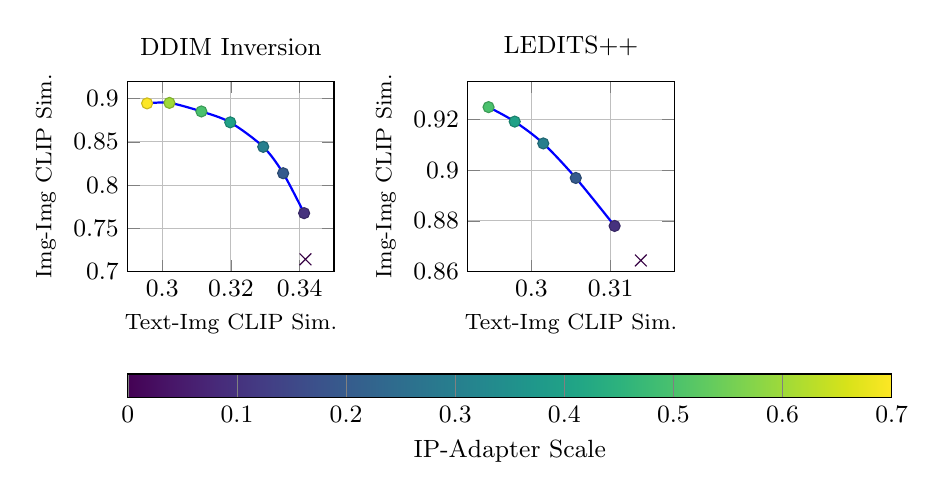
\begin{tikzpicture}
    \small{
    \begin{axis}[
        hide axis,
        scale only axis,
        height=0pt,
        colorbar horizontal,
        colormap/viridis, %
        colorbar style={
            width=0.8\linewidth, %
            height=0.3cm,
            yshift=-1cm,
            xlabel={IP-Adapter Scale}, %
            xticklabel style={/pgf/number format/.cd, fixed, precision=2},
        },
        point meta min=0.0, %
        point meta max=0.7, %
    ]
    \end{axis}

    \begin{axis}[
        name=plot1,
        width=4.2cm, height=4.0cm,
        xlabel={\footnotesize{Text-Img CLIP Sim.}},
        ylabel={\footnotesize{Img-Img CLIP Sim.}},
        title={DDIM Inversion},
        xmin=0.29, xmax=0.35,
        ymin=0.7, ymax=0.92,
        grid=both,
        legend pos=north west,
        colormap/viridis,
        colorbar=false, %
        point meta min=0.0, %
        point meta max=0.7, %
    ]
        \addplot[
            scatter,
            only marks,
            mark=*,
            mark size=2pt,
            scatter src=explicit, %
        ] table [meta=colormap] { %
            x       y       colormap
            0.3413  0.7676  0.1
            0.3352  0.8137  0.2
            0.3294  0.8442  0.3
            0.3198  0.8725  0.4
            0.3114  0.8851  0.5
            0.3021  0.8950  0.6
            0.2956  0.8944  0.7
        };

        \addplot[
            scatter,
            only marks,
            mark=x, %
            mark size=3pt, %
            scatter src=explicit,
        ] table [meta=colormap] {
            x       y       colormap
            0.3417  0.7143  0.0
        };
        
        \addplot[
            smooth,
            thick,
            blue,
        ] table {
            x       y
            0.3413  0.7676
            0.3352  0.8137
            0.3294  0.8442
            0.3198  0.8725
            0.3114  0.8851
            0.3021  0.8950
            0.2956  0.8944
        };
    \end{axis}

    \hspace{8pt}
    \begin{axis}[
        name=plot2,
        at=(plot1.right of south east), anchor=left of south west,
        width=4.2cm, height=4.0cm,
        xlabel={\footnotesize{Text-Img CLIP Sim.}},
        ylabel={\footnotesize{Img-Img CLIP Sim.}},
        title={LEDITS++},
        xmin=0.292, xmax=0.318,
        ymin=0.86, ymax=0.935,
        grid=both,
        legend pos=north west,
        colormap/viridis,
        colorbar=false, %
        point meta min=0.0, %
        point meta max=0.7, %
    ]
        \addplot[
            scatter,
            only marks,
            mark=*,
            mark size=2pt,
            scatter src=explicit, %
        ] table [meta=colormap] { %
            x       y       colormap
            0.3105  0.8780  0.1
            0.3056  0.8969  0.2
            0.3015  0.9105  0.3
            0.2979  0.9191  0.4
            0.2946  0.9248  0.5
        };

        \addplot[
            scatter,
            only marks,
            mark=x, %
            mark size=3pt, %
            scatter src=explicit,
        ] table [meta=colormap] {
            x       y       colormap
            0.3138  0.8644  0.0
        };
        
        \addplot[
            smooth,
            thick,
            blue,
        ] table {
            x       y
            0.3105  0.8780
            0.3056  0.8969
            0.3015  0.9105
            0.2979  0.9191
            0.2946  0.9248
        };
    \end{axis}
    }
\end{tikzpicture}

    \caption{CLIP Similarity of the edited text prompt and the edited image vs. CLIP Similarity of the source image and edited imaged for IPA scales in the range of 0 (without tight inversion, marked with a cross) to 0.7 (strong conditioning on the source image). For both axes, higher is better.}
    \label{fig:clip_similarity}
\end{figure}

\begin{figure}
    \centering
    \setlength{\tabcolsep}{1pt}
    \scriptsize{
    \begin{tabular}{cccccc}
        \multicolumn{5}{c}{``people in a diner'' $\longrightarrow$ ``robots in a diner'', DDIM Inversion} \\
        \includegraphics[width=0.195\linewidth]{images/compare_ddim/diner/original.jpg} &
        \includegraphics[width=0.195\linewidth]{images/masa/diner/reconstruction.jpg} &
        \includegraphics[width=0.195\linewidth]{images/masa/diner/reconstruction_ipa.jpg} &
        \includegraphics[width=0.195\linewidth]{images/compare_ddim/diner/edit.jpg} &
        \includegraphics[width=0.195\linewidth]{images/compare_ddim/diner/diner_edit_ipa.jpg} \\
        \multicolumn{5}{c}{``an antelope in the field'' $\longrightarrow$ ``... jumping in the field'', DDIM Inversion} \\
        \includegraphics[width=0.195\linewidth]{images/ddim/antilope/original.jpg} &
        \includegraphics[width=0.195\linewidth]{images/ddim/antilope/recon_ddim.jpg} &
        \includegraphics[width=0.195\linewidth]{images/ddim/antilope/recon_ours.jpg} &
        \includegraphics[width=0.195\linewidth]{images/ddim/antilope/jumping_ddim.jpg} &
        \includegraphics[width=0.195\linewidth]{images/ddim/antilope/jumping_ours.jpg} \\
        \multicolumn{5}{c}{``a dog in the snow'' $\longrightarrow$ ``a cat in the snow'', prompt2prompt} \\
        \includegraphics[width=0.195\linewidth]{images/p2p/dog_in_snow_ptp/original.jpg} &
        \includegraphics[width=0.195\linewidth]{images/p2p/dog_in_snow_ptp/reconstruction_no_ipa.jpg} &
        \includegraphics[width=0.195\linewidth]{images/p2p/dog_in_snow_ptp/reconstruction_ipa.jpg} &
        \includegraphics[width=0.195\linewidth]{images/p2p/dog_in_snow_ptp/cat_no_ipa.jpg} &
        \includegraphics[width=0.195\linewidth]{images/p2p/dog_in_snow_ptp/cat_ipa.jpg} \\
        \multicolumn{5}{c}{``a person'' $\longrightarrow$ ``a person with a thick beard'', Edit Friendly DDPM Inversion} \\
        \includegraphics[width=0.195\linewidth]{images/edit_friendly/man_holding_head/original.jpg} &
        \includegraphics[width=0.195\linewidth]{images/edit_friendly/man_holding_head/recon_ef.jpg} &
        \includegraphics[width=0.195\linewidth]{images/edit_friendly/man_holding_head/recon_ours.jpg} &
        \includegraphics[width=0.195\linewidth]{images/edit_friendly/man_holding_head/edit_ef_0.36.jpg} &
        \includegraphics[width=0.195\linewidth]{images/edit_friendly/man_holding_head/edit_ours_0.36_0.4.jpg} \\
        \multicolumn{5}{c}{``a wooden horse in the room'' $\longrightarrow$ ``a horse made of lego ...'', LEDITS++} \\
        \includegraphics[width=0.195\linewidth]{images/ledits/wooden_horse/wooden_horse_original.jpg} &
        \includegraphics[width=0.195\linewidth]{images/ledits/wooden_horse/wooden_horse_original.jpg} &
        \includegraphics[width=0.195\linewidth]{images/ledits/wooden_horse/wooden_horse_original.jpg} &
        \includegraphics[width=0.195\linewidth]{images/ledits/wooden_horse/lego_horse_no_ipa.jpg} &
        \includegraphics[width=0.195\linewidth]{images/ledits/wooden_horse/lego_horse_ipa.jpg} \\
        \multicolumn{5}{c}{``'' $\longrightarrow$ ``A portrait of an elf'', RF-Inversion (Flux)} \\
        \includegraphics[width=0.195\linewidth]{images/flux/masoud-elf/original.jpg}
        &
        \includegraphics[width=0.195\linewidth]{images/flux/masoud-elf/reconstruction.jpg} &
        \includegraphics[width=0.195\linewidth]{images/flux/masoud-elf/reconstruction_pulid.jpg} &
        \includegraphics[width=0.195\linewidth]{images/flux/masoud-elf/a_portrait_of_an_elf.jpg} &
        \includegraphics[width=0.195\linewidth]{images/flux/masoud-elf/a_portrait_of_an_elf_pulid.jpg} \\
        \multicolumn{5}{c}{``'' $\longrightarrow$ ``A portrait of a vampire'', RF-Inversion (Flux)} \\
        \includegraphics[width=0.195\linewidth]{images/flux/kolkatar-vampire/original.jpg}
        &
        \includegraphics[width=0.195\linewidth]{images/flux/kolkatar-vampire/reconstruction.jpg} &
        \includegraphics[width=0.195\linewidth]{images/flux/kolkatar-vampire/reconstruction_pulid.jpg} &
        \includegraphics[width=0.195\linewidth]{images/flux/kolkatar-vampire/a_portrait_of_a_vampire.jpg} &
        \includegraphics[width=0.195\linewidth]{images/flux/kolkatar-vampire/a_portrait_of_a_vampire_pulid.jpg} \\
        \multicolumn{5}{c}{``'' $\longrightarrow$ ``A bearded man wearing a hat'', RF-Inversion (Flux)} \\
        \includegraphics[width=0.195\linewidth]{images/flux/lecun/original.jpg} &
        \includegraphics[width=0.195\linewidth]{images/flux/lecun/reconstruction.jpg} &
        \includegraphics[width=0.195\linewidth]{images/flux/lecun/reconstruction_pulid.jpg} &
        \includegraphics[width=0.195\linewidth]{images/flux/lecun/A_bearded_man_wearing_a_hat.jpg} &
        \includegraphics[width=0.195\linewidth]{images/flux/lecun/A_bearded_man_wearing_a_hat_pulid.jpg} \\
        Input & Rec. w/o Tight & Rec. w/ Tight & Edit. w/o Tight & Edit. w/ Tight \\
    \end{tabular}
    }
    \caption{Combining Tight Inversion with various editing methods improves editability even in cases where the gap in reconstruction is negligible. Our method improves baseline methods for various editing types such as object addition, semantic modification, and pose modification.}
    \label{fig:edit-qualitative-comp}
\end{figure}


\paragraph{\textbf{Qualitative Comparison}}
We present qualitative results obtained with SDXL \cite{podell2024sdxl} and Flux~\cite{flux} in Figure~\ref{fig:edit-qualitative-comp} (more results are in Figures~\ref{fig:more-results1} and \ref{fig:more-results2}). In the first and second rows, we perform a na\"ive edit by changing the prompt during the denoising process. 
In the third row, we apply DDIM inversion and denoise the inverted noise using prompt2prompt \cite{hertz2022prompt}. 
The next two rows utilize the inversion and denoising methods from Edit Friendly DDPM \cite{hubermanspiegelglas2024editfriendlyddpmnoise} and LEDITS++ \cite{brack2024ledits}, respectievly.
In the last three rows, we use RF-Inversion \cite{rout2024rfinversion} with Flux, and we use PulID \cite{guo2024pulid} as the conditioning mechanism for our Tight Inversion method.
In each row, we show the input image, followed by the reconstruction results (with and without Tight Inversion), and then the edited images obtained from the inverted noises (with and without Tight Inversion).

Note that both Edit Friendly DDPM Inversion and LEDITS++ guarantee perfect reconstruction. For the other methods, we select examples where the reconstruction, even without Tight Inversion, is accurate. This choice emphasizes that, even when competing methods produce plausible reconstructions, our method outperforms them in terms of editability.

As shown in the results, our method better preserves the original image, maintaining the structure of the diner in the first row, the patterns on the snow and the animal's expression in the third row, and the horse's pose in the fifth row. In the results obtained with Flux, our method preserves the identity of the individual significantly better in the edited image, even when the reconstruction is comparable (e.g., the shape of LeCun's head). 


In Figure~\ref{fig:turbo_results}, we present results with SDXL-Turbo~\cite{sauer2023adversarialdiffusiondistillation}. Here, we use ReNoise inversion~\cite{garibi2024renoise} combined with Tight Inversion. To edit the inverted noise, we denoise it with a target text prompt. As shown, Tight Inversion results in better preservation of the cups in the top example and the background in the bottom example.

\begin{figure}
    \centering
    \setlength{\tabcolsep}{1pt}
    \scriptsize{
    \begin{tabular}{cccccc}
        \multicolumn{5}{c}{``A picture of tea cups'' $\longrightarrow$ ``... white tea cups''} \\
        \includegraphics[width=0.195\linewidth]{images/challenging_edits/cups/original.jpg} &
        \includegraphics[width=0.195\linewidth]{images/challenging_edits/cups/reconstruction.jpg} &
        \includegraphics[width=0.195\linewidth]{images/challenging_edits/cups/ipa/reconstruction.jpg} &
        \includegraphics[width=0.195\linewidth]{images/challenging_edits/cups/a_picture_of_white_tea_cups.jpg} &
        \includegraphics[width=0.195\linewidth]{images/challenging_edits/cups/ipa/a_picture_of_white_tea_cups.jpg} \\
        \multicolumn{5}{c}{``A woman is pulling a red suitcase down the sidewalk'' $\longrightarrow$} \\
        \multicolumn{5}{c}{ ``A woman is walking her dog and...''} \\
        \includegraphics[width=0.195\linewidth]{images/challenging_edits/163866/_ddim_renoise_turbo_split_3_163866_original.jpg} &
        \includegraphics[width=0.195\linewidth]{images/challenging_edits/163866/_ddim_renoise_turbo_split_3_163866_original_reconstruction_reconstruction.jpg} &
        \includegraphics[width=0.195\linewidth]{images/challenging_edits/163866/_ddim_renoise_turbo+ipa_split_3_163866_original_reconstruction_reconstruction.jpg} &
        \includegraphics[width=0.195\linewidth]{images/challenging_edits/163866/_ddim_renoise_turbo_split_3_163866_original_editing_0_A_woman_is_walking_her_dog_and_pulling_a_red_suitcase_down_the_sidewalk..jpg} &
        \includegraphics[width=0.195\linewidth]{images/challenging_edits/163866/_ddim_renoise_turbo+ipa_split_3_163866_original_editing_0_A_woman_is_walking_her_dog_and_pulling_a_red_suitcase_down_the_sidewalk..jpg} \\
        Input & Recon. w/o TiTi & Recon. w/ TiTi & Edit. w/o TiTi & Edit. w/ TiTi \\
    \end{tabular}
    }
    \caption{Combining Tight Inversion with ReNoise, where using SDXL-Turbo with 4 steps of denoising. The edit is applied by using a modified prompt in the denoising process.}
    \label{fig:turbo_results}
\end{figure}





\paragraph{\textbf{Quantitative Comparisons}}
Next, we evaluate our editing results quantitatively. We use the MagicBrush benchmark~\cite{Zhang2023MagicBrush} for the evaluation, as it contains diverse and challenging images and edits. Following previous work~\cite{brooks2023instructpix2pixlearningfollowimage} we evaluate the edit quality in terms of the preservation of the input image, and the adherence to the target prompt, and we use CLIP~\cite{radford2021learning} to measure both.
We present the results with DDIM Inversion and LEDITS++ in Figure~\ref{fig:clip_similarity}. In both graphs the tradeoff between image preservation and adherence to the target edit is clearly observed~\cite{tov2021designing}. Tight Inversion provides better control on this tradeoff, and better preserves the input image while still aligning with the edit prompt as also evident in Figure~\ref{fig:edit-qualitative-comp}. Note, that a CLIP similarity of above 0.3 between an image and a text prompt indicates plausible alignment between the image and the prompt. 


\paragraph{\textbf{Ablation Studies}}
In Figure~\ref{fig:ablation1}, we edit the image by denoising using a modified prompt. In the first row, where we use a random noise, the resulting image significantly differs from the input. In the second row, where the inversion is not conditioned on the input image, the red hat is not added, which may result from the initial noise being slightly out of distribution. This makes it more difficult to edit, particularly when an image condition is used. In the third row, a red hat is added to the man while the input image is successfully preserved.


We explore the IP-Adapter guidance scale effect on the edit in Figure~\ref{fig:ablation2}. In the third row, we add a cowboy hat to the deer, where various guidance scales are used for the inversion and denoising. 
We observe a clear reconstruction-editability tradeoff associated with the IP-Adapter scale. While increasing the scale improves reconstruction quality, it progressively limits editing capabilities, eventually preserving the original image intact. In practice, we found that an IP-Adapter scale of 0.4 strikes an effective balance for most cases.


